\batchmode
\documentclass[a4paper]{article}
\RequirePackage{ifthen}




\usepackage{array,amsmath,amssymb,rotating,graphicx}


\PassOptionsToPackage{colorlinks=true,linkcolor=blue,citecolor=blue,urlcolor=blue}{hyperref}
\usepackage{html}


\usepackage[dvips]{color}

\pagecolor[gray]{1.0}%
\providecommand{\HREF}[2]{\htmladdnormallink{#2}{#1}}%
\providecommand{\href}[2]{\htmladdnormallink{#2}{#1}} 

%
\providecommand{\MakeTutorialTitle}[1]{
\title{Tutorial: #1}
\begin{rawhtml}
<h1>\end{rawhtml}

#1
\begin{rawhtml}
</h1>
A Tutorial for the Course <em>Computational Intelligence</em>\end{rawhtml}



} 

%
\providecommand{\mat}[1]{{\tt >> #1} \\}%
\providecommand{\com}[1]{{\tt #1}} 

%
\providecommand{\tab}{\hspace{1em}} 

%
\providecommand{\trn}{^{\mathsf T}}  % transposition%
\providecommand{\xv}{\ensuremath\mathbf{x}}   % vector x%
\providecommand{\muv}{\ensuremath\boldsymbol{\mu}}   % vector mu%
\providecommand{\Sm}{\ensuremath\boldsymbol{\Sigma}}   % matrix Sigma%
\providecommand{\Tm}{\ensuremath\boldsymbol{\Theta}}   % matrix Sigma%
\providecommand{\Rf}{\ensuremath\mathbb{R}} 



\setlength{\hoffset}{-1in} 

\setlength{\voffset}{-1in} 



\setlength{\topskip}{0cm} 

\setlength{\headheight}{0cm} 

\setlength{\headsep}{0cm} 



\setlength{\textwidth}{16cm} 

\setlength{\evensidemargin}{2.5cm} 

\setlength{\oddsidemargin}{2.5cm} 



\setlength{\textheight}{24cm} 

\setlength{\topmargin}{2.5cm} 

\setlength{\headheight}{0.5cm} 

\setlength{\headsep}{0.5cm} 




\usepackage[latin1]{inputenc}



\makeatletter

\makeatletter
\count@=\the\catcode`\_ \catcode`\_=8 
\newenvironment{tex2html_wrap}{}{}%
\catcode`\<=12\catcode`\_=\count@
\newcommand{\providedcommand}[1]{\expandafter\providecommand\csname #1\endcsname}%
\newcommand{\renewedcommand}[1]{\expandafter\providecommand\csname #1\endcsname{}%
  \expandafter\renewcommand\csname #1\endcsname}%
\newcommand{\newedenvironment}[1]{\newenvironment{#1}{}{}\renewenvironment{#1}}%
\let\newedcommand\renewedcommand
\let\renewedenvironment\newedenvironment
\makeatother
\let\mathon=$
\let\mathoff=$
\ifx\AtBeginDocument\undefined \newcommand{\AtBeginDocument}[1]{}\fi
\newbox\sizebox
\setlength{\hoffset}{0pt}\setlength{\voffset}{0pt}
\addtolength{\textheight}{\footskip}\setlength{\footskip}{0pt}
\addtolength{\textheight}{\topmargin}\setlength{\topmargin}{0pt}
\addtolength{\textheight}{\headheight}\setlength{\headheight}{0pt}
\addtolength{\textheight}{\headsep}\setlength{\headsep}{0pt}
\setlength{\textwidth}{451pt}
\setlength{\textheight}{554pt}
\newwrite\lthtmlwrite
\makeatletter
\let\realnormalsize=\normalsize
\global\topskip=2sp
\def\preveqno{}\let\real@float=\@float \let\realend@float=\end@float
\def\@float{\let\@savefreelist\@freelist\real@float}
\def\liih@math{\ifmmode$\else\bad@math\fi}
\def\end@float{\realend@float\global\let\@freelist\@savefreelist}
\let\real@dbflt=\@dbflt \let\end@dblfloat=\end@float
\let\@largefloatcheck=\relax
\let\if@boxedmulticols=\iftrue
\def\@dbflt{\let\@savefreelist\@freelist\real@dbflt}
\def\adjustnormalsize{\def\normalsize{\mathsurround=0pt \realnormalsize
 \parindent=0pt\abovedisplayskip=0pt\belowdisplayskip=0pt}%
 \def\phantompar{\csname par\endcsname}\normalsize}%
\def\lthtmltypeout#1{{\let\protect\string \immediate\write\lthtmlwrite{#1}}}%
\newcommand\lthtmlhboxmathA{\adjustnormalsize\setbox\sizebox=\hbox\bgroup\kern.05em }%
\newcommand\lthtmlhboxmathB{\adjustnormalsize\setbox\sizebox=\hbox to\hsize\bgroup\hfill }%
\newcommand\lthtmlvboxmathA{\adjustnormalsize\setbox\sizebox=\vbox\bgroup %
 \let\ifinner=\iffalse \let\)\liih@math }%
\newcommand\lthtmlboxmathZ{\@next\next\@currlist{}{\def\next{\voidb@x}}%
 \expandafter\box\next\egroup}%
\newcommand\lthtmlmathtype[1]{\gdef\lthtmlmathenv{#1}}%
\newcommand\lthtmllogmath{\lthtmltypeout{l2hSize %
:\lthtmlmathenv:\the\ht\sizebox::\the\dp\sizebox::\the\wd\sizebox.\preveqno}}%
\newcommand\lthtmlfigureA[1]{\let\@savefreelist\@freelist
       \lthtmlmathtype{#1}\lthtmlvboxmathA}%
\newcommand\lthtmlpictureA{\bgroup\catcode`\_=8 \lthtmlpictureB}%
\newcommand\lthtmlpictureB[1]{\lthtmlmathtype{#1}\egroup
       \let\@savefreelist\@freelist \lthtmlhboxmathB}%
\newcommand\lthtmlpictureZ[1]{\hfill\lthtmlfigureZ}%
\newcommand\lthtmlfigureZ{\lthtmlboxmathZ\lthtmllogmath\copy\sizebox
       \global\let\@freelist\@savefreelist}%
\newcommand\lthtmldisplayA{\bgroup\catcode`\_=8 \lthtmldisplayAi}%
\newcommand\lthtmldisplayAi[1]{\lthtmlmathtype{#1}\egroup\lthtmlvboxmathA}%
\newcommand\lthtmldisplayB[1]{\edef\preveqno{(\theequation)}%
  \lthtmldisplayA{#1}\let\@eqnnum\relax}%
\newcommand\lthtmldisplayZ{\lthtmlboxmathZ\lthtmllogmath\lthtmlsetmath}%
\newcommand\lthtmlinlinemathA{\bgroup\catcode`\_=8 \lthtmlinlinemathB}
\newcommand\lthtmlinlinemathB[1]{\lthtmlmathtype{#1}\egroup\lthtmlhboxmathA
  \vrule height1.5ex width0pt }%
\newcommand\lthtmlinlineA{\bgroup\catcode`\_=8 \lthtmlinlineB}%
\newcommand\lthtmlinlineB[1]{\lthtmlmathtype{#1}\egroup\lthtmlhboxmathA}%
\newcommand\lthtmlinlineZ{\egroup\expandafter\ifdim\dp\sizebox>0pt %
  \expandafter\centerinlinemath\fi\lthtmllogmath\lthtmlsetinline}
\newcommand\lthtmlinlinemathZ{\egroup\expandafter\ifdim\dp\sizebox>0pt %
  \expandafter\centerinlinemath\fi\lthtmllogmath\lthtmlsetmath}
\newcommand\lthtmlindisplaymathZ{\egroup %
  \centerinlinemath\lthtmllogmath\lthtmlsetmath}
\def\lthtmlsetinline{\hbox{\vrule width.1em \vtop{\vbox{%
  \kern.1em\copy\sizebox}\ifdim\dp\sizebox>0pt\kern.1em\else\kern.3pt\fi
  \ifdim\hsize>\wd\sizebox \hrule depth1pt\fi}}}
\def\lthtmlsetmath{\hbox{\vrule width.1em\kern-.05em\vtop{\vbox{%
  \kern.1em\kern0.7 pt\hbox{\hglue.17em\copy\sizebox\hglue0.7 pt}}\kern.3pt%
  \ifdim\dp\sizebox>0pt\kern.1em\fi \kern0.7 pt%
  \ifdim\hsize>\wd\sizebox \hrule depth1pt\fi}}}
\def\centerinlinemath{%
  \dimen1=\ifdim\ht\sizebox<\dp\sizebox \dp\sizebox\else\ht\sizebox\fi
  \advance\dimen1by.5pt \vrule width0pt height\dimen1 depth\dimen1 
 \dp\sizebox=\dimen1\ht\sizebox=\dimen1\relax}

\def\lthtmlcheckvsize{\ifdim\ht\sizebox<\vsize 
  \ifdim\wd\sizebox<\hsize\expandafter\hfill\fi \expandafter\vfill
  \else\expandafter\vss\fi}%
\providecommand{\selectlanguage}[1]{}%
\makeatletter \tracingstats = 1 
\providecommand{\Eta}{\textrm{H}}
\providecommand{\Mu}{\textrm{M}}
\providecommand{\Alpha}{\textrm{A}}
\providecommand{\Iota}{\textrm{J}}
\providecommand{\Nu}{\textrm{N}}
\providecommand{\Omicron}{\textrm{O}}
\providecommand{\omicron}{\textrm{o}}
\providecommand{\Chi}{\textrm{X}}
\providecommand{\Beta}{\textrm{B}}
\providecommand{\Kappa}{\textrm{K}}
\providecommand{\Tau}{\textrm{T}}
\providecommand{\Epsilon}{\textrm{E}}
\providecommand{\Zeta}{\textrm{Z}}
\providecommand{\Rho}{\textrm{R}}


\begin{document}
\pagestyle{empty}\thispagestyle{empty}\lthtmltypeout{}%
\lthtmltypeout{latex2htmlLength hsize=\the\hsize}\lthtmltypeout{}%
\lthtmltypeout{latex2htmlLength vsize=\the\vsize}\lthtmltypeout{}%
\lthtmltypeout{latex2htmlLength hoffset=\the\hoffset}\lthtmltypeout{}%
\lthtmltypeout{latex2htmlLength voffset=\the\voffset}\lthtmltypeout{}%
\lthtmltypeout{latex2htmlLength topmargin=\the\topmargin}\lthtmltypeout{}%
\lthtmltypeout{latex2htmlLength topskip=\the\topskip}\lthtmltypeout{}%
\lthtmltypeout{latex2htmlLength headheight=\the\headheight}\lthtmltypeout{}%
\lthtmltypeout{latex2htmlLength headsep=\the\headsep}\lthtmltypeout{}%
\lthtmltypeout{latex2htmlLength parskip=\the\parskip}\lthtmltypeout{}%
\lthtmltypeout{latex2htmlLength oddsidemargin=\the\oddsidemargin}\lthtmltypeout{}%
\makeatletter
\if@twoside\lthtmltypeout{latex2htmlLength evensidemargin=\the\evensidemargin}%
\else\lthtmltypeout{latex2htmlLength evensidemargin=\the\oddsidemargin}\fi%
\lthtmltypeout{}%
\makeatother
\setcounter{page}{1}
\onecolumn

% !!! IMAGES START HERE !!!

{\newpage\clearpage
\lthtmlinlinemathA{tex2html_wrap_inline3226}%
$ {\cal  N}(\ensuremath  \boldsymbol  {\mu }_{\text  {/i/}},\ensuremath  \boldsymbol  {\Sigma }_{\text  {/i/}})$%
\lthtmlinlinemathZ
\lthtmlcheckvsize\clearpage}

{\newpage\clearpage
\lthtmlinlinemathA{tex2html_wrap_inline3228}%
$ {\cal  N}(\ensuremath  \boldsymbol  {\mu }_{\text  {/e/}},\ensuremath  \boldsymbol  {\Sigma }_{\text  {/e/}})$%
\lthtmlinlinemathZ
\lthtmlcheckvsize\clearpage}

{\newpage\clearpage
\lthtmlinlinemathA{tex2html_wrap_inline3230}%
$ {\cal  N}(\ensuremath  \boldsymbol  {\mu }_{\text  {/i/}},\ensuremath  \boldsymbol  {\Sigma }_{\text  {/e/}})$%
\lthtmlinlinemathZ
\lthtmlcheckvsize\clearpage}

{\newpage\clearpage
\lthtmlinlinemathA{tex2html_wrap_inline3236}%
$ K$%
\lthtmlinlinemathZ
\lthtmlcheckvsize\clearpage}

\stepcounter{section}
\stepcounter{subsection}
{\newpage\clearpage
\lthtmlinlinemathA{tex2html_wrap_inline3247}%
$ d$%
\lthtmlinlinemathZ
\lthtmlcheckvsize\clearpage}

{\newpage\clearpage
\lthtmlinlinemathA{tex2html_wrap_inline3249}%
$ \ensuremath\mathbf{x}\circlearrowleft {\cal
N}(\ensuremath\boldsymbol{\mu},\ensuremath\boldsymbol{\Sigma})$%
\lthtmlinlinemathZ
\lthtmlcheckvsize\clearpage}

{\newpage\clearpage
\lthtmlinlinemathA{tex2html_wrap_inline3251}%
$ \ensuremath\mathbf{x}\in \ensuremath\mathbb{R}^d$%
\lthtmlinlinemathZ
\lthtmlcheckvsize\clearpage}

{\newpage\clearpage
\lthtmlinlinemathA{tex2html_wrap_indisplay3253}%
$\displaystyle g_{(\ensuremath\boldsymbol{\mu},\ensuremath\boldsymbol{\Sigma})}(\ensuremath\mathbf{x}) = \frac{1}{\sqrt{2\pi}^d
       \sqrt{\det\left(\ensuremath\boldsymbol{\Sigma}\right)}} \, e^{-\frac{1}{2} (\ensuremath\mathbf{x}-\ensuremath\boldsymbol{\mu})^{\mathsf T}
       \ensuremath\boldsymbol{\Sigma}^{-1} (\ensuremath\mathbf{x}-\ensuremath\boldsymbol{\mu})}$%
\lthtmlindisplaymathZ
\lthtmlcheckvsize\clearpage}

{\newpage\clearpage
\lthtmlinlinemathA{tex2html_wrap_inline3255}%
$ \ensuremath\boldsymbol{\mu}$%
\lthtmlinlinemathZ
\lthtmlcheckvsize\clearpage}

{\newpage\clearpage
\lthtmlinlinemathA{tex2html_wrap_inline3257}%
$ \ensuremath\boldsymbol{\Sigma}$%
\lthtmlinlinemathZ
\lthtmlcheckvsize\clearpage}

{\newpage\clearpage
\lthtmlinlinemathA{tex2html_wrap_inline3265}%
$ \mu_i = E(x_i)$%
\lthtmlinlinemathZ
\lthtmlcheckvsize\clearpage}

{\newpage\clearpage
\lthtmlinlinemathA{tex2html_wrap_inline3267}%
$ E(x)$%
\lthtmlinlinemathZ
\lthtmlcheckvsize\clearpage}

{\newpage\clearpage
\lthtmlinlinemathA{tex2html_wrap_inline3269}%
$ x$%
\lthtmlinlinemathZ
\lthtmlcheckvsize\clearpage}

{\newpage\clearpage
\lthtmlinlinemathA{tex2html_wrap_inline3271}%
$ c_{ii}$%
\lthtmlinlinemathZ
\lthtmlcheckvsize\clearpage}

{\newpage\clearpage
\lthtmlinlinemathA{tex2html_wrap_inline3273}%
$ c_{ij}$%
\lthtmlinlinemathZ
\lthtmlcheckvsize\clearpage}

{\newpage\clearpage
\lthtmlinlinemathA{tex2html_wrap_inline3277}%
$ d\times d$%
\lthtmlinlinemathZ
\lthtmlcheckvsize\clearpage}

{\newpage\clearpage
\lthtmlinlinemathA{tex2html_wrap_indisplay3279}%
$\displaystyle \ensuremath\boldsymbol{\Sigma}=
   \left[
     \begin{array}{*{4}{c}}
       c_{11} & c_{12} & \cdots & c_{1n} \\
       c_{21} & c_{22} & \cdots & c_{2n} \\
       \vdots & \vdots & \ddots & \vdots \\
       c_{n1} & c_{n2} & \cdots & c_{nn} \\
     \end{array}
   \right]$%
\lthtmlindisplaymathZ
\lthtmlcheckvsize\clearpage}

{\newpage\clearpage
\lthtmlinlinemathA{tex2html_wrap_inline3283}%
$ x_i$%
\lthtmlinlinemathZ
\lthtmlcheckvsize\clearpage}

{\newpage\clearpage
\lthtmlinlinemathA{tex2html_wrap_inline3285}%
$ x_j$%
\lthtmlinlinemathZ
\lthtmlcheckvsize\clearpage}

{\newpage\clearpage
\lthtmlinlinemathA{tex2html_wrap_inline3287}%
$ \ensuremath\mathbf{x}$%
\lthtmlinlinemathZ
\lthtmlcheckvsize\clearpage}

{\newpage\clearpage
\lthtmlinlinemathA{tex2html_wrap_indisplay3289}%
$\displaystyle c_{ij} = E\left((x_i-\mu_i)^{\mathsf T}\,(x_j-\mu_j)\right).$%
\lthtmlindisplaymathZ
\lthtmlcheckvsize\clearpage}

{\newpage\clearpage
\lthtmlinlinemathA{tex2html_wrap_inline3295}%
$ i\ne j$%
\lthtmlinlinemathZ
\lthtmlcheckvsize\clearpage}

{\newpage\clearpage
\lthtmlinlinemathA{tex2html_wrap_inline3297}%
$ c_{ij} = 0$%
\lthtmlinlinemathZ
\lthtmlcheckvsize\clearpage}

{\newpage\clearpage
\lthtmlinlinemathA{tex2html_wrap_inline3301}%
$ \sqrt{\ensuremath\boldsymbol{\Sigma}}$%
\lthtmlinlinemathZ
\lthtmlcheckvsize\clearpage}

{\newpage\clearpage
\lthtmlinlinemathA{tex2html_wrap_inline3305}%
$ \ensuremath\mathbf{x}\circlearrowleft {\cal N}(\mathbf{0},\mathbf{I})$%
\lthtmlinlinemathZ
\lthtmlcheckvsize\clearpage}

{\newpage\clearpage
\lthtmlinlinemathA{tex2html_wrap_inline3309}%
$ \mathbf{I}$%
\lthtmlinlinemathZ
\lthtmlcheckvsize\clearpage}

{\newpage\clearpage
\lthtmlinlinemathA{tex2html_wrap_inline3311}%
$ \mathbf{y} = \ensuremath\boldsymbol{\mu}+
\sqrt{\ensuremath\boldsymbol{\Sigma}}\,\ensuremath\mathbf{x}$%
\lthtmlinlinemathZ
\lthtmlcheckvsize\clearpage}

{\newpage\clearpage
\lthtmlinlinemathA{tex2html_wrap_inline3313}%
$ \mathbf{y} \circlearrowleft {\cal
N}(\ensuremath\boldsymbol{\mu},\ensuremath\boldsymbol{\Sigma})$%
\lthtmlinlinemathZ
\lthtmlcheckvsize\clearpage}

\stepcounter{subsubsection}
{\newpage\clearpage
\lthtmlinlinemathA{tex2html_wrap_inline3316}%
$ X$%
\lthtmlinlinemathZ
\lthtmlcheckvsize\clearpage}

{\newpage\clearpage
\lthtmlinlinemathA{tex2html_wrap_inline3318}%
$ N$%
\lthtmlinlinemathZ
\lthtmlcheckvsize\clearpage}

{\newpage\clearpage
\lthtmlinlinemathA{tex2html_wrap_inline3320}%
$ X=\{\ensuremath\mathbf{x}_1,
\ensuremath\mathbf{x}_2,\ldots,\ensuremath\mathbf{x}_N\}$%
\lthtmlinlinemathZ
\lthtmlcheckvsize\clearpage}

{\newpage\clearpage
\lthtmlinlinemathA{tex2html_wrap_inline3322}%
$ N=10000$%
\lthtmlinlinemathZ
\lthtmlcheckvsize\clearpage}

{\newpage\clearpage
\lthtmlinlinemathA{tex2html_wrap_indisplay3324}%
$\displaystyle \ensuremath\boldsymbol{\mu}= \left[ \begin{array}{c} 730 \\1090 \end{array} \right]
$%
\lthtmlindisplaymathZ
\lthtmlcheckvsize\clearpage}

{\newpage\clearpage
\lthtmlinlinemathA{tex2html_wrap_inline3326}%
$ X_1$%
\lthtmlinlinemathZ
\lthtmlcheckvsize\clearpage}

{\newpage\clearpage
\lthtmlinlinemathA{tex2html_wrap_indisplay3328}%
$\displaystyle \ensuremath\boldsymbol{\Sigma}_1 = \left[ \begin{array}{cc}
8000 & 0 \\
0    & 8000
\end{array} \right]
$%
\lthtmlindisplaymathZ
\lthtmlcheckvsize\clearpage}

{\newpage\clearpage
\lthtmlinlinemathA{tex2html_wrap_inline3330}%
$ X_2$%
\lthtmlinlinemathZ
\lthtmlcheckvsize\clearpage}

{\newpage\clearpage
\lthtmlinlinemathA{tex2html_wrap_indisplay3332}%
$\displaystyle \ensuremath\boldsymbol{\Sigma}_2 = \left[ \begin{array}{cc}
8000 & 0 \\
0    & 18500
\end{array} \right]
$%
\lthtmlindisplaymathZ
\lthtmlcheckvsize\clearpage}

{\newpage\clearpage
\lthtmlinlinemathA{tex2html_wrap_inline3334}%
$ X_3$%
\lthtmlinlinemathZ
\lthtmlcheckvsize\clearpage}

{\newpage\clearpage
\lthtmlinlinemathA{tex2html_wrap_indisplay3336}%
$\displaystyle \ensuremath\boldsymbol{\Sigma}_3 = \left[ \begin{array}{cc}
8000 & 8400 \\
8400 & 18500
\end{array} \right]
$%
\lthtmlindisplaymathZ
\lthtmlcheckvsize\clearpage}

{\newpage\clearpage
\lthtmlinlinemathA{tex2html_wrap_inline3339}%
$ \ensuremath\boldsymbol{\Sigma}_2$%
\lthtmlinlinemathZ
\lthtmlcheckvsize\clearpage}

{\newpage\clearpage
\lthtmlinlinemathA{tex2html_wrap_inline3341}%
$ \ensuremath\boldsymbol{\Sigma}_3$%
\lthtmlinlinemathZ
\lthtmlcheckvsize\clearpage}

{\newpage\clearpage
\lthtmlinlinemathA{tex2html_wrap_inline3343}%
$ \circlearrowleft$%
\lthtmlinlinemathZ
\lthtmlcheckvsize\clearpage}

{\newpage\clearpage
\lthtmlinlinemathA{tex2html_wrap_inline3360}%
$ \Box$%
\lthtmlinlinemathZ
\lthtmlcheckvsize\clearpage}

{\newpage\clearpage
\lthtmlinlinemathA{tex2html_wrap_inline3362}%
$ \ensuremath\mathbf{x}_i$%
\lthtmlinlinemathZ
\lthtmlcheckvsize\clearpage}

{\newpage\clearpage
\lthtmlinlinemathA{tex2html_wrap_inline3384}%
$ c_{ij} = c_{ji}$%
\lthtmlinlinemathZ
\lthtmlcheckvsize\clearpage}

{\newpage\clearpage
\lthtmlinlinemathA{tex2html_wrap_inline3388}%
$ \ensuremath\mathbf{x}^{\mathsf T}\ensuremath\boldsymbol{\Sigma}\, \ensuremath\mathbf{x}\ge 0$%
\lthtmlinlinemathZ
\lthtmlcheckvsize\clearpage}

\stepcounter{subsection}
{\newpage\clearpage
\lthtmlinlinemathA{tex2html_wrap_inline3403}%
$ \displaystyle \hat{\ensuremath\boldsymbol{\mu}} = \frac{1}{N}
\sum_{i=1}^{N} \ensuremath\mathbf{x}_i$%
\lthtmlinlinemathZ
\lthtmlcheckvsize\clearpage}

{\newpage\clearpage
\lthtmlinlinemathA{tex2html_wrap_inline3405}%
$ \displaystyle \hat{\ensuremath\boldsymbol{\Sigma}} =
\frac{1}{N-1} \; \sum_{i=1}^{N} (\ensuremath\mathbf{x}_i-\ensuremath\boldsymbol{\mu})^{\mathsf T}(\ensuremath\mathbf{x}_i-\ensuremath\boldsymbol{\mu}) $%
\lthtmlinlinemathZ
\lthtmlcheckvsize\clearpage}

\stepcounter{subsubsection}
{\newpage\clearpage
\lthtmlinlinemathA{tex2html_wrap_inline3410}%
$ {\cal
N}(\ensuremath\boldsymbol{\mu},\ensuremath\boldsymbol{\Sigma}_3)$%
\lthtmlinlinemathZ
\lthtmlcheckvsize\clearpage}

{\newpage\clearpage
\lthtmlinlinemathA{tex2html_wrap_inline3412}%
$ \hat{\ensuremath\boldsymbol{\mu}}$%
\lthtmlinlinemathZ
\lthtmlcheckvsize\clearpage}

{\newpage\clearpage
\lthtmlinlinemathA{tex2html_wrap_inline3414}%
$ \hat{\ensuremath\boldsymbol{\Sigma}}$%
\lthtmlinlinemathZ
\lthtmlcheckvsize\clearpage}

{\newpage\clearpage
\lthtmlinlinemathA{tex2html_wrap_inline3416}%
$ \hat{\ensuremath\boldsymbol{\mu}}_{(10000)}
=$%
\lthtmlinlinemathZ
\lthtmlcheckvsize\clearpage}

{\newpage\clearpage
\lthtmlinlinemathA{tex2html_wrap_inline3418}%
$ \hat{\ensuremath\boldsymbol{\Sigma}}_{(10000)} =$%
\lthtmlinlinemathZ
\lthtmlcheckvsize\clearpage}

{\newpage\clearpage
\lthtmlinlinemathA{tex2html_wrap_inline3420}%
$ \hat{\ensuremath\boldsymbol{\mu}}_{(1000)}
=$%
\lthtmlinlinemathZ
\lthtmlcheckvsize\clearpage}

{\newpage\clearpage
\lthtmlinlinemathA{tex2html_wrap_inline3422}%
$ \hat{\ensuremath\boldsymbol{\Sigma}}_{(1000)} =$%
\lthtmlinlinemathZ
\lthtmlcheckvsize\clearpage}

{\newpage\clearpage
\lthtmlinlinemathA{tex2html_wrap_inline3424}%
$ \hat{\ensuremath\boldsymbol{\mu}}_{(100)}
=$%
\lthtmlinlinemathZ
\lthtmlcheckvsize\clearpage}

{\newpage\clearpage
\lthtmlinlinemathA{tex2html_wrap_inline3426}%
$ \hat{\ensuremath\boldsymbol{\Sigma}}_{(100)} =$%
\lthtmlinlinemathZ
\lthtmlcheckvsize\clearpage}

{\newpage\clearpage
\lthtmlinlinemathA{tex2html_wrap_inline3436}%
$ \|\mathbf{A}-\mathbf{B}\|_2$%
\lthtmlinlinemathZ
\lthtmlcheckvsize\clearpage}

{\newpage\clearpage
\lthtmlinlinemathA{tex2html_wrap_inline3438}%
$ \mathbf{A}$%
\lthtmlinlinemathZ
\lthtmlcheckvsize\clearpage}

{\newpage\clearpage
\lthtmlinlinemathA{tex2html_wrap_inline3440}%
$ \mathbf{B}$%
\lthtmlinlinemathZ
\lthtmlcheckvsize\clearpage}

\stepcounter{subsubsection}
\stepcounter{subsubsection}
\stepcounter{subsection}
{\newpage\clearpage
\lthtmlinlinemathA{tex2html_wrap_inline3466}%
$ \ensuremath\boldsymbol{\Theta}$%
\lthtmlinlinemathZ
\lthtmlcheckvsize\clearpage}

{\newpage\clearpage
\lthtmlinlinemathA{tex2html_wrap_inline3473}%
$ p(\ensuremath\mathbf{x}_i|\ensuremath\boldsymbol{\Theta})$%
\lthtmlinlinemathZ
\lthtmlcheckvsize\clearpage}

{\newpage\clearpage
\lthtmlinlinemathA{tex2html_wrap_inline3475}%
$ \ensuremath\boldsymbol{\Theta}= (\ensuremath\boldsymbol{\mu},\ensuremath\boldsymbol{\Sigma})$%
\lthtmlinlinemathZ
\lthtmlcheckvsize\clearpage}

{\newpage\clearpage
\lthtmlinlinemathA{tex2html_wrap_indisplay3479}%
$\displaystyle p(X|\ensuremath\boldsymbol{\Theta}) =
     \prod_{i=1}^{N} p(\ensuremath\mathbf{x}_i|\ensuremath\boldsymbol{\Theta}) =
     \prod_{i=1}^{N} p(\ensuremath\mathbf{x}_i|\ensuremath\boldsymbol{\mu},\ensuremath\boldsymbol{\Sigma}) =
     \prod_{i=1}^{N} g_{(\ensuremath\boldsymbol{\mu},\ensuremath\boldsymbol{\Sigma})}(\ensuremath\mathbf{x}_i)$%
\lthtmlindisplaymathZ
\lthtmlcheckvsize\clearpage}

\stepcounter{subsubsection}
{\newpage\clearpage
\lthtmlinlinemathA{tex2html_wrap_indisplay3482}%
$\displaystyle p(X|\ensuremath\boldsymbol{\Theta}) = \prod_{i=1}^{N} p(\ensuremath\mathbf{x}_i|\ensuremath\boldsymbol{\Theta}) \quad \Leftrightarrow \quad
\log p(X|\ensuremath\boldsymbol{\Theta}) = \log \prod_{i=1}^{N} p(\ensuremath\mathbf{x}_i|\ensuremath\boldsymbol{\Theta}) = \sum_{i=1}^{N}
\log p(\ensuremath\mathbf{x}_i|\ensuremath\boldsymbol{\Theta})
$%
\lthtmlindisplaymathZ
\lthtmlcheckvsize\clearpage}

{\newpage\clearpage
\lthtmlinlinemathA{tex2html_wrap_indisplay3485}%
$\displaystyle p(\ensuremath\mathbf{x}|\ensuremath\boldsymbol{\Theta})$%
\lthtmlindisplaymathZ
\lthtmlcheckvsize\clearpage}

{\newpage\clearpage
\lthtmlinlinemathA{tex2html_wrap_indisplay3487}%
$\displaystyle =$%
\lthtmlindisplaymathZ
\lthtmlcheckvsize\clearpage}

{\newpage\clearpage
\lthtmlinlinemathA{tex2html_wrap_indisplay3489}%
$\displaystyle \frac{1}{\sqrt{2\pi}^d \sqrt{\det\left(\ensuremath\boldsymbol{\Sigma}\right)}}
\, e^{-\frac{1}{2} (\ensuremath\mathbf{x}-\ensuremath\boldsymbol{\mu})^{\mathsf T}\ensuremath\boldsymbol{\Sigma}^{-1} (\ensuremath\mathbf{x}-\ensuremath\boldsymbol{\mu})}$%
\lthtmlindisplaymathZ
\lthtmlcheckvsize\clearpage}

{\newpage\clearpage
\lthtmlinlinemathA{tex2html_wrap_indisplay3491}%
$\displaystyle \log p(\ensuremath\mathbf{x}|\ensuremath\boldsymbol{\Theta})$%
\lthtmlindisplaymathZ
\lthtmlcheckvsize\clearpage}

{\newpage\clearpage
\lthtmlinlinemathA{tex2html_wrap_indisplay3495}%
$\displaystyle \frac{1}{2} \left[-d \log \left( 2\pi \right)
-  \log \left( \det\left(\ensuremath\boldsymbol{\Sigma}\right) \right)
-  (\ensuremath\mathbf{x}-\ensuremath\boldsymbol{\mu})^{\mathsf T}\ensuremath\boldsymbol{\Sigma}^{-1} (\ensuremath\mathbf{x}-\ensuremath\boldsymbol{\mu})\right]$%
\lthtmlindisplaymathZ
\lthtmlcheckvsize\clearpage}

{\newpage\clearpage
\lthtmlinlinemathA{tex2html_wrap_inline3497}%
$ \log(x)$%
\lthtmlinlinemathZ
\lthtmlcheckvsize\clearpage}

{\newpage\clearpage
\lthtmlinlinemathA{tex2html_wrap_indisplay3499}%
$\displaystyle p(x|\ensuremath\boldsymbol{\Theta}_1) > p(x|\ensuremath\boldsymbol{\Theta}_2) \quad \Leftrightarrow \quad
\log p(x|\ensuremath\boldsymbol{\Theta}_1) > \log p(x|\ensuremath\boldsymbol{\Theta}_2),
$%
\lthtmlindisplaymathZ
\lthtmlcheckvsize\clearpage}

{\newpage\clearpage
\lthtmlinlinemathA{tex2html_wrap_inline3509}%
$ \frac{1}{2}
\left[\ldots\right]$%
\lthtmlinlinemathZ
\lthtmlcheckvsize\clearpage}

{\newpage\clearpage
\lthtmlinlinemathA{tex2html_wrap_inline3513}%
$ d\log \left( 2\pi \right)$%
\lthtmlinlinemathZ
\lthtmlcheckvsize\clearpage}

{\newpage\clearpage
\lthtmlinlinemathA{tex2html_wrap_inline3517}%
$ \log \left( \det\left(\ensuremath\boldsymbol{\Sigma}\right)
\right)$%
\lthtmlinlinemathZ
\lthtmlcheckvsize\clearpage}

{\newpage\clearpage
\lthtmlinlinemathA{tex2html_wrap_inline3521}%
$ (\ensuremath\mathbf{x}-\ensuremath\boldsymbol{\mu})^{\mathsf T}\ensuremath\boldsymbol{\Sigma}^{-1} (\ensuremath\mathbf{x}-\ensuremath\boldsymbol{\mu})$%
\lthtmlinlinemathZ
\lthtmlcheckvsize\clearpage}

\stepcounter{subsubsection}
{\newpage\clearpage
\lthtmlinlinemathA{tex2html_wrap_inline3547}%
$ \ensuremath\boldsymbol{\Theta}_i = (\ensuremath\boldsymbol{\mu}_i,\ensuremath\boldsymbol{\Sigma}_i)$%
\lthtmlinlinemathZ
\lthtmlcheckvsize\clearpage}

{\newpage\clearpage
\lthtmlinlinemathA{tex2html_wrap_inline3549}%
$ {\cal N}_1: \; \ensuremath\boldsymbol{\Theta}_1 = \left(
\left[\begin{array}{c}730 \\1090\end{array}\right],
\left[\begin{array}{cc}8000 & 0 \\0 & 8000\end{array}\right]
\right)$%
\lthtmlinlinemathZ
\lthtmlcheckvsize\clearpage}

{\newpage\clearpage
\lthtmlinlinemathA{tex2html_wrap_inline3551}%
$ {\cal N}_2: \; \ensuremath\boldsymbol{\Theta}_2 = \left(
\left[\begin{array}{c}730 \\1090\end{array}\right],
\left[\begin{array}{cc}8000 & 0 \\0 & 18500\end{array}\right]
\right)$%
\lthtmlinlinemathZ
\lthtmlcheckvsize\clearpage}

{\newpage\clearpage
\lthtmlinlinemathA{tex2html_wrap_inline3553}%
$ {\cal N}_3: \; \ensuremath\boldsymbol{\Theta}_3 = \left(
\left[\begin{array}{c}730 \\1090\end{array}\right],
\left[\begin{array}{cc}8000 & 8400 \\8400 & 18500\end{array}\right]
\right)$%
\lthtmlinlinemathZ
\lthtmlcheckvsize\clearpage}

{\newpage\clearpage
\lthtmlinlinemathA{tex2html_wrap_inline3555}%
$ {\cal N}_4: \; \ensuremath\boldsymbol{\Theta}_4 = \left(
\left[\begin{array}{c}270 \\1690\end{array}\right],
\left[\begin{array}{cc}8000 & 8400 \\8400 & 18500\end{array}\right]
\right)$%
\lthtmlinlinemathZ
\lthtmlcheckvsize\clearpage}

{\newpage\clearpage
\lthtmlinlinemathA{tex2html_wrap_indisplay3565}%
$\displaystyle \log p(X_3|\ensuremath\boldsymbol{\Theta}_1),\; \log p(X_3|\ensuremath\boldsymbol{\Theta}_2),\; \log p(X_3|\ensuremath\boldsymbol{\Theta}_3),\;$%
\lthtmlindisplaymathZ
\lthtmlcheckvsize\clearpage}

{\newpage\clearpage
\lthtmlinlinemathA{tex2html_wrap_indisplay3566}%
$\displaystyle \; \log p(X_3|\ensuremath\boldsymbol{\Theta}_4).
$%
\lthtmlindisplaymathZ
\lthtmlcheckvsize\clearpage}

\stepcounter{subsubsection}
{\newpage\clearpage
\lthtmlinlinemathA{tex2html_wrap_inline3569}%
$ {\cal N}_1$%
\lthtmlinlinemathZ
\lthtmlcheckvsize\clearpage}

{\newpage\clearpage
\lthtmlinlinemathA{tex2html_wrap_inline3571}%
$ {\cal N}_2$%
\lthtmlinlinemathZ
\lthtmlcheckvsize\clearpage}

{\newpage\clearpage
\lthtmlinlinemathA{tex2html_wrap_inline3573}%
$ {\cal
N}_3$%
\lthtmlinlinemathZ
\lthtmlcheckvsize\clearpage}

{\newpage\clearpage
\lthtmlinlinemathA{tex2html_wrap_inline3575}%
$ {\cal N}_4$%
\lthtmlinlinemathZ
\lthtmlcheckvsize\clearpage}

\stepcounter{section}
\stepcounter{subsection}
\stepcounter{subsubsection}
{\newpage\clearpage
\lthtmlinlinemathA{tex2html_wrap_inline3593}%
$ [F_1,F_2]$%
\lthtmlinlinemathZ
\lthtmlcheckvsize\clearpage}

{\newpage\clearpage
\lthtmlinlinemathA{tex2html_wrap_inline3597}%
$ N\times2$%
\lthtmlinlinemathZ
\lthtmlcheckvsize\clearpage}

{\newpage\clearpage
\lthtmlinlinemathA{tex2html_wrap_inline3601}%
$ P(q_k)$%
\lthtmlinlinemathZ
\lthtmlcheckvsize\clearpage}

{\newpage\clearpage
\lthtmlinlinemathA{tex2html_wrap_inline3603}%
$ q_k$%
\lthtmlinlinemathZ
\lthtmlcheckvsize\clearpage}

{\newpage\clearpage
\lthtmlinlinemathA{tex2html_wrap_inline3605}%
$ k \in
\{$%
\lthtmlinlinemathZ
\lthtmlcheckvsize\clearpage}

{\newpage\clearpage
\lthtmlinlinemathA{tex2html_wrap_inline3606}%
$ ,$%
\lthtmlinlinemathZ
\lthtmlcheckvsize\clearpage}

{\newpage\clearpage
\lthtmlinlinemathA{tex2html_wrap_inline3610}%
$ \}$%
\lthtmlinlinemathZ
\lthtmlcheckvsize\clearpage}

\stepcounter{subsubsection}
\stepcounter{subsection}
\stepcounter{subsubsection}
\stepcounter{subsection}
{\newpage\clearpage
\lthtmlinlinemathA{tex2html_wrap_indisplay3624}%
$\displaystyle X \in q_k$%
\lthtmlindisplaymathZ
\lthtmlcheckvsize\clearpage}

{\newpage\clearpage
\lthtmlinlinemathA{tex2html_wrap_indisplay3625}%
$\displaystyle \quad P(q_k|X,\ensuremath\boldsymbol{\Theta}) \geq P(q_j|X,\ensuremath\boldsymbol{\Theta}),
\quad\forall j \neq k
$%
\lthtmlindisplaymathZ
\lthtmlcheckvsize\clearpage}

{\newpage\clearpage
\lthtmlinlinemathA{tex2html_wrap_inline3635}%
$ P(q_k|X,\ensuremath\boldsymbol{\Theta})$%
\lthtmlinlinemathZ
\lthtmlcheckvsize\clearpage}

{\newpage\clearpage
\lthtmlinlinemathA{tex2html_wrap_inline3637}%
$ P(q_k|\ensuremath\boldsymbol{\Theta})$%
\lthtmlinlinemathZ
\lthtmlcheckvsize\clearpage}

{\newpage\clearpage
\lthtmlinlinemathA{tex2html_wrap_indisplay3645}%
$\displaystyle P(q_k|X,\ensuremath\boldsymbol{\Theta}) = \frac{p(X|q_k,\ensuremath\boldsymbol{\Theta})\; P(q_k|\ensuremath\boldsymbol{\Theta})}{p(X|\ensuremath\boldsymbol{\Theta})}$%
\lthtmlindisplaymathZ
\lthtmlcheckvsize\clearpage}

{\newpage\clearpage
\lthtmlinlinemathA{tex2html_wrap_inline3653}%
$ p(X|\ensuremath\boldsymbol{\Theta})=$%
\lthtmlinlinemathZ
\lthtmlcheckvsize\clearpage}

{\newpage\clearpage
\lthtmlinlinemathA{tex2html_wrap_inline3659}%
$ p(X|q_k,\ensuremath\boldsymbol{\Theta}) P(q_k|\ensuremath\boldsymbol{\Theta})$%
\lthtmlinlinemathZ
\lthtmlcheckvsize\clearpage}

{\newpage\clearpage
\lthtmlinlinemathA{tex2html_wrap_indisplay3661}%
$\displaystyle P(q_k|X,\ensuremath\boldsymbol{\Theta}) \propto p(X|q_k,\ensuremath\boldsymbol{\Theta})\; P(q_k|\ensuremath\boldsymbol{\Theta}), \quad \forall k
$%
\lthtmlindisplaymathZ
\lthtmlcheckvsize\clearpage}

{\newpage\clearpage
\lthtmlinlinemathA{tex2html_wrap_inline3663}%
$ \log$%
\lthtmlinlinemathZ
\lthtmlcheckvsize\clearpage}

{\newpage\clearpage
\lthtmlinlinemathA{tex2html_wrap_indisplay3665}%
$\displaystyle \log P(q_k|X,\ensuremath\boldsymbol{\Theta}) \propto \log p(X|q_k,\ensuremath\boldsymbol{\Theta}) + \log P(q_k|\ensuremath\boldsymbol{\Theta})$%
\lthtmlindisplaymathZ
\lthtmlcheckvsize\clearpage}

{\newpage\clearpage
\lthtmlinlinemathA{tex2html_wrap_inline3669}%
$ \ensuremath\boldsymbol{\mu}_k$%
\lthtmlinlinemathZ
\lthtmlcheckvsize\clearpage}

{\newpage\clearpage
\lthtmlinlinemathA{tex2html_wrap_inline3671}%
$ \ensuremath\boldsymbol{\Sigma}_k$%
\lthtmlinlinemathZ
\lthtmlcheckvsize\clearpage}

{\newpage\clearpage
\lthtmlinlinemathA{tex2html_wrap_inline3677}%
$ ,/u/\}$%
\lthtmlinlinemathZ
\lthtmlcheckvsize\clearpage}

{\newpage\clearpage
\lthtmlinlinemathA{tex2html_wrap_inline3679}%
$ p(X|q_k,\ensuremath\boldsymbol{\Theta})$%
\lthtmlinlinemathZ
\lthtmlcheckvsize\clearpage}

{\newpage\clearpage
\lthtmlinlinemathA{tex2html_wrap_inline3681}%
$ \log p(X|q_k,\ensuremath\boldsymbol{\Theta})$%
\lthtmlinlinemathZ
\lthtmlcheckvsize\clearpage}

{\newpage\clearpage
\lthtmlinlinemathA{tex2html_wrap_inline3689}%
$ (\ensuremath\boldsymbol{\mu}_k,\ensuremath\boldsymbol{\Sigma}_k)$%
\lthtmlinlinemathZ
\lthtmlcheckvsize\clearpage}

\stepcounter{subsubsection}
{\newpage\clearpage
\lthtmlinlinemathA{tex2html_wrap_inline3712}%
$ p(X|\ensuremath\boldsymbol{\Theta})$%
\lthtmlinlinemathZ
\lthtmlcheckvsize\clearpage}

{\newpage\clearpage
\lthtmlinlinemathA{tex2html_wrap_inline3720}%
$ \ensuremath\mathbf{x}_i=[F_1,F_2]^{\mathsf T}$%
\lthtmlinlinemathZ
\lthtmlcheckvsize\clearpage}

{\newpage\clearpage
\lthtmlinlinemathA{tex2html_wrap_inline3722}%
$ f_k(\ensuremath\mathbf{x}_i)$%
\lthtmlinlinemathZ
\lthtmlcheckvsize\clearpage}

{\newpage\clearpage
\lthtmlinlinemathA{tex2html_wrap_inline3726}%
$ f_k(\ensuremath\mathbf{x}_i) = \log
p(\ensuremath\mathbf{x}_i|q_k,\ensuremath\boldsymbol{\Theta}) + \log P(q_k|\ensuremath\boldsymbol{\Theta})$%
\lthtmlinlinemathZ
\lthtmlcheckvsize\clearpage}


\renewcommand{\arraystretch}{1.5}


\setlength{\tabcolsep}{0.12in}%

\setlength{\tabcolsep}{0.12in}
{\newpage\clearpage
\lthtmlinlinemathA{tex2html_wrap_inline3734}%
$ f_{\text{/a/}}(\ensuremath\mathbf{x}_i)$%
\lthtmlinlinemathZ
\lthtmlcheckvsize\clearpage}

{\newpage\clearpage
\lthtmlinlinemathA{tex2html_wrap_inline3736}%
$ f_{\text{/e/}}(\ensuremath\mathbf{x}_i)$%
\lthtmlinlinemathZ
\lthtmlcheckvsize\clearpage}

{\newpage\clearpage
\lthtmlinlinemathA{tex2html_wrap_inline3738}%
$ f_{\text{/i/}}(\ensuremath\mathbf{x}_i)$%
\lthtmlinlinemathZ
\lthtmlcheckvsize\clearpage}

{\newpage\clearpage
\lthtmlinlinemathA{tex2html_wrap_inline3740}%
$ f_{\text{/o/}}(\ensuremath\mathbf{x}_i)$%
\lthtmlinlinemathZ
\lthtmlcheckvsize\clearpage}

{\newpage\clearpage
\lthtmlinlinemathA{tex2html_wrap_inline3742}%
$ f_{\text{/y/}}(\ensuremath\mathbf{x}_i)$%
\lthtmlinlinemathZ
\lthtmlcheckvsize\clearpage}

{\newpage\clearpage
\lthtmlinlinemathA{tex2html_wrap_inline3746}%
$ [400,1800]^{\mathsf T}$%
\lthtmlinlinemathZ
\lthtmlcheckvsize\clearpage}

{\newpage\clearpage
\lthtmlinlinemathA{tex2html_wrap_inline3748}%
$ [400,1000]^{\mathsf T}$%
\lthtmlinlinemathZ
\lthtmlcheckvsize\clearpage}

{\newpage\clearpage
\lthtmlinlinemathA{tex2html_wrap_inline3750}%
$ [530,1000]^{\mathsf T}$%
\lthtmlinlinemathZ
\lthtmlcheckvsize\clearpage}

{\newpage\clearpage
\lthtmlinlinemathA{tex2html_wrap_inline3752}%
$ [600,1300]^{\mathsf T}$%
\lthtmlinlinemathZ
\lthtmlcheckvsize\clearpage}

{\newpage\clearpage
\lthtmlinlinemathA{tex2html_wrap_inline3754}%
$ [670,1300]^{\mathsf T}$%
\lthtmlinlinemathZ
\lthtmlcheckvsize\clearpage}

{\newpage\clearpage
\lthtmlinlinemathA{tex2html_wrap_inline3756}%
$ [420,2500]^{\mathsf T}$%
\lthtmlinlinemathZ
\lthtmlcheckvsize\clearpage}

\stepcounter{subsubsection}
{\newpage\clearpage
\lthtmlinlinemathA{tex2html_wrap_inline3815}%
$ \log p(\ensuremath\mathbf{x}_i|q_k,\ensuremath\boldsymbol{\Theta})$%
\lthtmlinlinemathZ
\lthtmlcheckvsize\clearpage}

{\newpage\clearpage
\lthtmlinlinemathA{tex2html_wrap_inline3819}%
$ x_1$%
\lthtmlinlinemathZ
\lthtmlcheckvsize\clearpage}

\stepcounter{subsection}
{\newpage\clearpage
\lthtmlinlinemathA{tex2html_wrap_inline3826}%
$ d-1$%
\lthtmlinlinemathZ
\lthtmlcheckvsize\clearpage}

{\newpage\clearpage
\lthtmlinlinemathA{tex2html_wrap_inline3833}%
$ f_k(\ensuremath\mathbf{x})$%
\lthtmlinlinemathZ
\lthtmlcheckvsize\clearpage}

{\newpage\clearpage
\lthtmlinlinemathA{tex2html_wrap_inline3837}%
$ k$%
\lthtmlinlinemathZ
\lthtmlcheckvsize\clearpage}

{\newpage\clearpage
\lthtmlinlinemathA{tex2html_wrap_indisplay3841}%
$\displaystyle \ensuremath\mathbf{x}\in q_k \quad \Leftrightarrow \quad f_k(\ensuremath\mathbf{x},\ensuremath\boldsymbol{\Theta}_k) \geq f_l(\ensuremath\mathbf{x},\ensuremath\boldsymbol{\Theta}_l),
\quad \forall l \neq k
$%
\lthtmlindisplaymathZ
\lthtmlcheckvsize\clearpage}

{\newpage\clearpage
\lthtmlinlinemathA{tex2html_wrap_inline3847}%
$ P(q_k|\ensuremath\mathbf{x}_i)$%
\lthtmlinlinemathZ
\lthtmlcheckvsize\clearpage}

{\newpage\clearpage
\lthtmlinlinemathA{tex2html_wrap_indisplay3854}%
$\displaystyle \ensuremath\mathbf{x}\in q_k$%
\lthtmlindisplaymathZ
\lthtmlcheckvsize\clearpage}

{\newpage\clearpage
\lthtmlinlinemathA{tex2html_wrap_indisplay3856}%
$\displaystyle \Leftrightarrow$%
\lthtmlindisplaymathZ
\lthtmlcheckvsize\clearpage}

{\newpage\clearpage
\lthtmlinlinemathA{tex2html_wrap_indisplay3858}%
$\displaystyle P(q_k|\ensuremath\mathbf{x}_i) \geq P(q_l|\ensuremath\mathbf{x}_i),\quad \forall l \neq k$%
\lthtmlindisplaymathZ
\lthtmlcheckvsize\clearpage}

{\newpage\clearpage
\lthtmlinlinemathA{tex2html_wrap_indisplay3862}%
$\displaystyle p(\ensuremath\mathbf{x}_i|q_k)\; P(q_k) \geq p(\ensuremath\mathbf{x}_i|q_l)\; P(q_l),\quad
\forall l \neq k$%
\lthtmlindisplaymathZ
\lthtmlcheckvsize\clearpage}

{\newpage\clearpage
\lthtmlinlinemathA{tex2html_wrap_indisplay3866}%
$\displaystyle \log p(\ensuremath\mathbf{x}_i|q_k)+\log P(q_k) \geq \log
p(\ensuremath\mathbf{x}_i|q_l)+\log P(q_l),\quad \forall l \neq k$%
\lthtmlindisplaymathZ
\lthtmlcheckvsize\clearpage}

\stepcounter{subsubsection}
{\newpage\clearpage
\lthtmlpictureA{tex2html_wrap3871}%
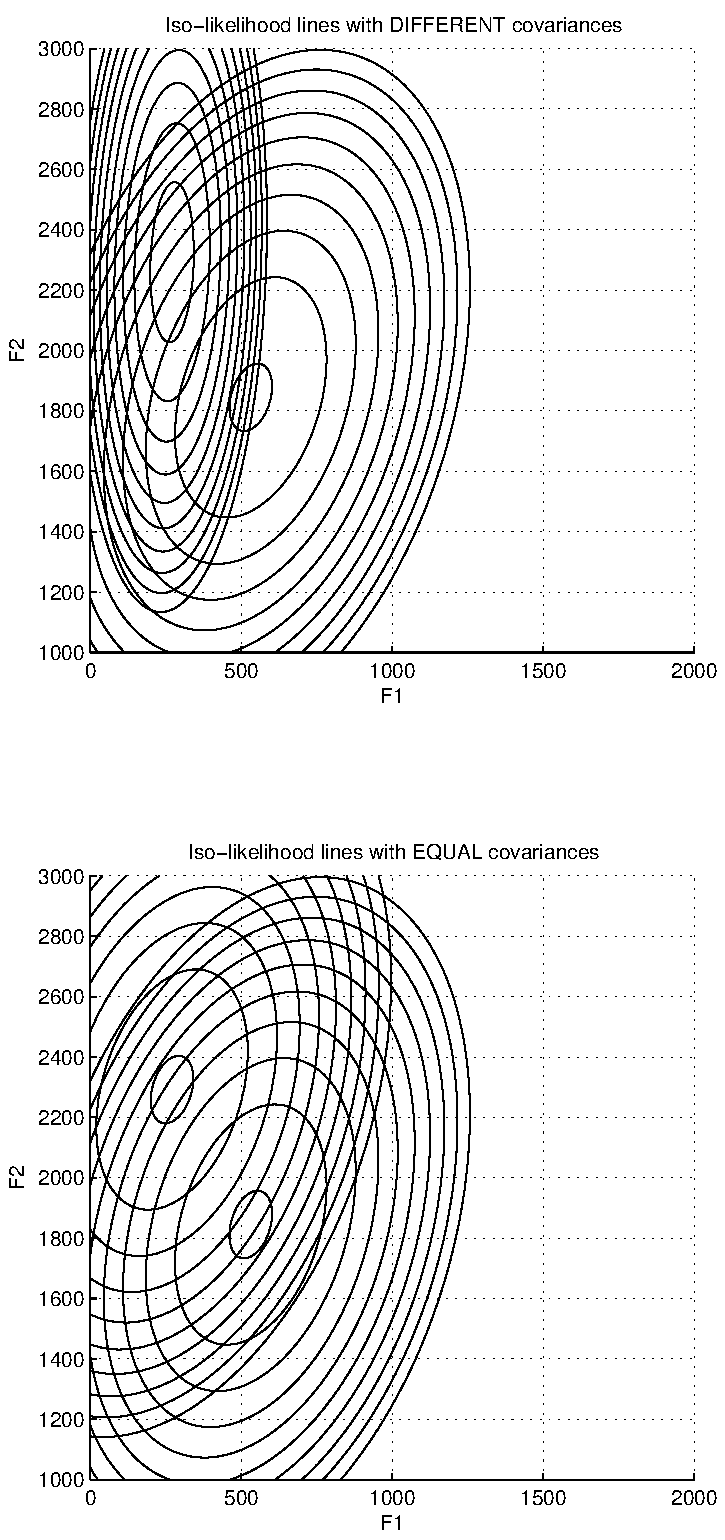
\includegraphics[height=0.95\textheight]{iso}%
\lthtmlpictureZ
\lthtmlcheckvsize\clearpage}

{\newpage\clearpage
\lthtmlinlinemathA{tex2html_wrap_inline3900}%
$ \ensuremath\boldsymbol{\Sigma}_{\text{/e/}}$%
\lthtmlinlinemathZ
\lthtmlcheckvsize\clearpage}

\stepcounter{subsubsection}
\stepcounter{section}
\stepcounter{subsection}
{\newpage\clearpage
\lthtmlinlinemathA{tex2html_wrap_inline3920}%
$ k=1,\ldots,K$%
\lthtmlinlinemathZ
\lthtmlcheckvsize\clearpage}

{\newpage\clearpage
\lthtmlinlinemathA{tex2html_wrap_inline3922}%
$ \ensuremath\mathbf{x}_n$%
\lthtmlinlinemathZ
\lthtmlcheckvsize\clearpage}

{\newpage\clearpage
\lthtmlinlinemathA{tex2html_wrap_inline3924}%
$ n=1,\ldots,N$%
\lthtmlinlinemathZ
\lthtmlcheckvsize\clearpage}

{\newpage\clearpage
\lthtmlinlinemathA{tex2html_wrap_inline3926}%
$ k^{\text{th}}$%
\lthtmlinlinemathZ
\lthtmlcheckvsize\clearpage}

{\newpage\clearpage
\lthtmlinlinemathA{tex2html_wrap_indisplay3929}%
$\displaystyle d_k(\ensuremath\mathbf{x}_n)$%
\lthtmlindisplaymathZ
\lthtmlcheckvsize\clearpage}

{\newpage\clearpage
\lthtmlinlinemathA{tex2html_wrap_indisplay3933}%
$\displaystyle \, \left\| \ensuremath\mathbf{x}_n - \ensuremath\boldsymbol{\mu}_k \right\|^2$%
\lthtmlindisplaymathZ
\lthtmlcheckvsize\clearpage}

{\newpage\clearpage
\lthtmlinlinemathA{tex2html_wrap_indisplay3937}%
$\displaystyle (\ensuremath\mathbf{x}_n-\ensuremath\boldsymbol{\mu}_k)^{\mathsf T}(\ensuremath\mathbf{x}_n-\ensuremath\boldsymbol{\mu}_k)$%
\lthtmlindisplaymathZ
\lthtmlcheckvsize\clearpage}

{\newpage\clearpage
\lthtmlinlinemathA{tex2html_wrap_indisplay3947}%
$\displaystyle d_k(\ensuremath\mathbf{x}_n) \, < \, d_l(\ensuremath\mathbf{x}_n), \qquad \forall l \neq k
$%
\lthtmlindisplaymathZ
\lthtmlcheckvsize\clearpage}

{\newpage\clearpage
\lthtmlinlinemathA{tex2html_wrap_indisplay3949}%
$\displaystyle J = \sum_{k=1}^{K} \sum_{\ensuremath\mathbf{x}_n \in q_k} d_k(\ensuremath\mathbf{x}_n)
$%
\lthtmlindisplaymathZ
\lthtmlcheckvsize\clearpage}

{\newpage\clearpage
\lthtmlinlinemathA{tex2html_wrap_inline3954}%
$ \{\ensuremath\boldsymbol{\mu}_{\text{/a/}},
\ensuremath\boldsymbol{\mu}_{\text{/e/}}, \ensuremath\boldsymbol{\mu}_{\text{/i/}}, \ensuremath\boldsymbol{\mu}_{\text{/o/}},
\ensuremath\boldsymbol{\mu}_{\text{/y/}}\}$%
\lthtmlinlinemathZ
\lthtmlcheckvsize\clearpage}

{\newpage\clearpage
\lthtmlinlinemathA{tex2html_wrap_inline3956}%
$ 2\times$%
\lthtmlinlinemathZ
\lthtmlcheckvsize\clearpage}

\stepcounter{subsection}
{\newpage\clearpage
\lthtmlinlinemathA{tex2html_wrap_inline3964}%
$ {\cal N}(\ensuremath\boldsymbol{\mu}_{k},\ensuremath\boldsymbol{\Sigma}_{k}),
\; k=1\ldots K$%
\lthtmlinlinemathZ
\lthtmlcheckvsize\clearpage}

{\newpage\clearpage
\lthtmlinlinemathA{tex2html_wrap_inline3972}%
$ k=1\ldots K$%
\lthtmlinlinemathZ
\lthtmlcheckvsize\clearpage}

{\newpage\clearpage
\lthtmlinlinemathA{tex2html_wrap_inline3976}%
$ 1/K$%
\lthtmlinlinemathZ
\lthtmlcheckvsize\clearpage}

{\newpage\clearpage
\lthtmlinlinemathA{tex2html_wrap_inline3978}%
$ Q$%
\lthtmlinlinemathZ
\lthtmlcheckvsize\clearpage}

{\newpage\clearpage
\lthtmlinlinemathA{tex2html_wrap_inline3986}%
$ p(X,Q|\ensuremath\boldsymbol{\Theta})$%
\lthtmlinlinemathZ
\lthtmlcheckvsize\clearpage}

{\newpage\clearpage
\lthtmlinlinemathA{tex2html_wrap_inline3994}%
$ i$%
\lthtmlinlinemathZ
\lthtmlcheckvsize\clearpage}

{\newpage\clearpage
\lthtmlinlinemathA{tex2html_wrap_indisplay3996}%
$\displaystyle \ensuremath\boldsymbol{\mu}_{k}^{(i+1)} =$%
\lthtmlindisplaymathZ
\lthtmlcheckvsize\clearpage}

{\newpage\clearpage
\lthtmlinlinemathA{tex2html_wrap_indisplay3997}%
$\displaystyle q_k^{(i)}
$%
\lthtmlindisplaymathZ
\lthtmlcheckvsize\clearpage}

{\newpage\clearpage
\lthtmlinlinemathA{tex2html_wrap_indisplay3999}%
$\displaystyle \ensuremath\boldsymbol{\Sigma}_{k}^{(i+1)} =$%
\lthtmlindisplaymathZ
\lthtmlcheckvsize\clearpage}

{\newpage\clearpage
\lthtmlinlinemathA{tex2html_wrap_indisplay4002}%
$\displaystyle P(q_k^{(i+1)}|\ensuremath\boldsymbol{\Theta}^{(i+1)}) = \frac{\mbox{number of training points
belonging to } q_k^{(i)} }{\mbox{total number of training points}}
$%
\lthtmlindisplaymathZ
\lthtmlcheckvsize\clearpage}

{\newpage\clearpage
\lthtmlinlinemathA{tex2html_wrap_indisplay4005}%
$\displaystyle {\cal L}(\ensuremath\boldsymbol{\Theta})$%
\lthtmlindisplaymathZ
\lthtmlcheckvsize\clearpage}

{\newpage\clearpage
\lthtmlinlinemathA{tex2html_wrap_indisplay4009}%
$\displaystyle \sum_{X} P(X|\ensuremath\boldsymbol{\Theta}) \;=\; \sum_{Q} \sum_{X} p(X,Q|\ensuremath\boldsymbol{\Theta})$%
\lthtmlindisplaymathZ
\lthtmlcheckvsize\clearpage}

{\newpage\clearpage
\lthtmlinlinemathA{tex2html_wrap_indisplay4013}%
$\displaystyle \sum_{k=1}^{K} \sum_{\ensuremath\mathbf{x}_n \in q_k} \log p(\ensuremath\mathbf{x}_n|\ensuremath\boldsymbol{\Theta}_k),$%
\lthtmlindisplaymathZ
\lthtmlcheckvsize\clearpage}

{\newpage\clearpage
\lthtmlinlinemathA{tex2html_wrap_inline4020}%
$ \{\ensuremath\boldsymbol{\Sigma}_{\text{/a/}}, \ensuremath\boldsymbol{\Sigma}_{\text{/e/}}, \ensuremath\boldsymbol{\Sigma}_{\text{/i/}},
\ensuremath\boldsymbol{\Sigma}_{\text{/o/}}, \ensuremath\boldsymbol{\Sigma}_{\text{/y/}}\}$%
\lthtmlinlinemathZ
\lthtmlcheckvsize\clearpage}

{\newpage\clearpage
\lthtmlinlinemathA{tex2html_wrap_inline4022}%
$ [P_{\text{/a/}},P_{\text{/e/}},P_{\text{/i/}},P_{\text{/o/}},P_{\text{/y/}}]$%
\lthtmlinlinemathZ
\lthtmlcheckvsize\clearpage}

\stepcounter{subsection}
{\newpage\clearpage
\lthtmlinlinemathA{tex2html_wrap_inline4030}%
$ P(q_k) = 1/K$%
\lthtmlinlinemathZ
\lthtmlcheckvsize\clearpage}

{\newpage\clearpage
\lthtmlinlinemathA{tex2html_wrap_inline4032}%
$ P(q_k^{(i)}|\ensuremath\mathbf{x}_n,\ensuremath\boldsymbol{\Theta}^{(i)})$%
\lthtmlinlinemathZ
\lthtmlcheckvsize\clearpage}

{\newpage\clearpage
\lthtmlinlinemathA{tex2html_wrap_inline4036}%
$ q_k^{(i)}$%
\lthtmlinlinemathZ
\lthtmlcheckvsize\clearpage}

{\newpage\clearpage
\lthtmlinlinemathA{tex2html_wrap_indisplay4039}%
$\displaystyle P(q_k^{(i)}|\ensuremath\mathbf{x}_n,\ensuremath\boldsymbol{\Theta}^{(i)})$%
\lthtmlindisplaymathZ
\lthtmlcheckvsize\clearpage}

{\newpage\clearpage
\lthtmlinlinemathA{tex2html_wrap_indisplay4043}%
$\displaystyle \frac{P(q_k^{(i)}|\ensuremath\boldsymbol{\Theta}^{(i)})
\cdot p(\ensuremath\mathbf{x}_n|q_k^{(i)},\ensuremath\boldsymbol{\Theta}^{(i)})}
{p(\ensuremath\mathbf{x}_n|\ensuremath\boldsymbol{\Theta}^{(i)})}$%
\lthtmlindisplaymathZ
\lthtmlcheckvsize\clearpage}

{\newpage\clearpage
\lthtmlinlinemathA{tex2html_wrap_indisplay4047}%
$\displaystyle \frac{P(q_k^{(i)}|\ensuremath\boldsymbol{\Theta}^{(i)}) \cdot p(\ensuremath\mathbf{x}_n|\ensuremath\boldsymbol{\mu}_k^{(i)},\ensuremath\boldsymbol{\Sigma}_k^{(i)}) }
{\sum_j P(q_j^{(i)}|\ensuremath\boldsymbol{\Theta}^{(i)}) \cdot p(\ensuremath\mathbf{x}_n|\ensuremath\boldsymbol{\mu}_j^{(i)},\ensuremath\boldsymbol{\Sigma}_j^{(i)}) }$%
\lthtmlindisplaymathZ
\lthtmlcheckvsize\clearpage}

{\newpage\clearpage
\lthtmlinlinemathA{tex2html_wrap_inline4051}%
$ [0,1]$%
\lthtmlinlinemathZ
\lthtmlcheckvsize\clearpage}

{\newpage\clearpage
\lthtmlinlinemathA{tex2html_wrap_indisplay4057}%
$\displaystyle \ensuremath\boldsymbol{\mu}_{k}^{(i+1)} = \frac{\sum_{n=1}^{N} \ensuremath\mathbf{x}_n
P(q_k^{(i)}|\ensuremath\mathbf{x}_n,\ensuremath\boldsymbol{\Theta}^{(i)})}
{\sum_{n=1}^{N} P(q_k^{(i)}|\ensuremath\mathbf{x}_n,\ensuremath\boldsymbol{\Theta}^{(i)})} $%
\lthtmlindisplaymathZ
\lthtmlcheckvsize\clearpage}

{\newpage\clearpage
\lthtmlinlinemathA{tex2html_wrap_indisplay4059}%
$\displaystyle \ensuremath\boldsymbol{\Sigma}_{k}^{(i+1)} = \frac{\sum_{n=1}^{N} P(q_k^{(i)}|\ensuremath\mathbf{x}_n,\ensuremath\boldsymbol{\Theta}^{(i)})\;
(\ensuremath\mathbf{x}_n - \ensuremath\boldsymbol{\mu}_k^{(i+1)})(\ensuremath\mathbf{x}_n - \ensuremath\boldsymbol{\mu}_k^{(i+1)})^{\mathsf T}}
{\sum_{n=1}^{N} P(q_k^{(i)}|\ensuremath\mathbf{x}_n,\ensuremath\boldsymbol{\Theta}^{(i)})} $%
\lthtmlindisplaymathZ
\lthtmlcheckvsize\clearpage}

{\newpage\clearpage
\lthtmlinlinemathA{tex2html_wrap_indisplay4061}%
$\displaystyle P(q_k^{(i+1)}|\ensuremath\boldsymbol{\Theta}^{(i+1)}) = \frac{1}{N} \sum_{n=1}^{N}
P(q_k^{(i)}|\ensuremath\mathbf{x}_n,\ensuremath\boldsymbol{\Theta}^{(i)}) $%
\lthtmlindisplaymathZ
\lthtmlcheckvsize\clearpage}

{\newpage\clearpage
\lthtmlinlinemathA{tex2html_wrap_indisplay4064}%
$\displaystyle {\cal L}(\ensuremath\boldsymbol{\Theta}) = \log p(X|\ensuremath\boldsymbol{\Theta})$%
\lthtmlindisplaymathZ
\lthtmlcheckvsize\clearpage}

{\newpage\clearpage
\lthtmlinlinemathA{tex2html_wrap_indisplay4065}%
$\displaystyle = \log \sum_Q p(X,Q|\ensuremath\boldsymbol{\Theta})$%
\lthtmlindisplaymathZ
\lthtmlcheckvsize\clearpage}

{\newpage\clearpage
\lthtmlinlinemathA{tex2html_wrap_indisplay4066}%
$\displaystyle = \log \sum_Q P(Q|X,\ensuremath\boldsymbol{\Theta})p(X|\ensuremath\boldsymbol{\Theta})$%
\lthtmlindisplaymathZ
\lthtmlcheckvsize\clearpage}

{\newpage\clearpage
\lthtmlinlinemathA{tex2html_wrap_indisplay4067}%
$\displaystyle = \log \sum_{k=1}^{K} P(q_k|X,\ensuremath\boldsymbol{\Theta}) p(X|\ensuremath\boldsymbol{\Theta})$%
\lthtmlindisplaymathZ
\lthtmlcheckvsize\clearpage}

{\newpage\clearpage
\lthtmlinlinemathA{tex2html_wrap_inline4069}%
$ \left( \log \sum_j \lambda_j y_j \geq
\sum_j \lambda_j \log y_j \mbox{ if } \sum_j \lambda_j = 1 \right)$%
\lthtmlinlinemathZ
\lthtmlcheckvsize\clearpage}

{\newpage\clearpage
\lthtmlinlinemathA{tex2html_wrap_indisplay4070}%
$\displaystyle {\cal L}(\ensuremath\boldsymbol{\Theta}) \ge J(\ensuremath\boldsymbol{\Theta})$%
\lthtmlindisplaymathZ
\lthtmlcheckvsize\clearpage}

{\newpage\clearpage
\lthtmlinlinemathA{tex2html_wrap_indisplay4071}%
$\displaystyle = \sum_{k=1}^{K} P(q_k|X,\ensuremath\boldsymbol{\Theta}) \log p(X|\ensuremath\boldsymbol{\Theta})$%
\lthtmlindisplaymathZ
\lthtmlcheckvsize\clearpage}

{\newpage\clearpage
\lthtmlinlinemathA{tex2html_wrap_indisplay4072}%
$\displaystyle = \sum_{k=1}^{K} \sum_{n=1}^{N} P(q_k|\ensuremath\mathbf{x}_n,\ensuremath\boldsymbol{\Theta}) \log p(\ensuremath\mathbf{x}_n|\ensuremath\boldsymbol{\Theta})$%
\lthtmlindisplaymathZ
\lthtmlcheckvsize\clearpage}

{\newpage\clearpage
\lthtmlinlinemathA{tex2html_wrap_inline4074}%
$ J(\ensuremath\boldsymbol{\Theta})$%
\lthtmlinlinemathZ
\lthtmlcheckvsize\clearpage}

{\newpage\clearpage
\lthtmlinlinemathA{tex2html_wrap_inline4076}%
$ {\cal
L}(\ensuremath\boldsymbol{\Theta})$%
\lthtmlinlinemathZ
\lthtmlcheckvsize\clearpage}


\end{document}
